\newcommand{\midheading}[1]{
	{ \vskip 1em \centering \large \textsc{#1} \par \vskip 1em }}







\newcommand{\sysname}[1]{"\textsc{#1}"}






\chapter{Post-Formalism in Constructed Memories}
\section{Post-Formalist Mathematics}

Over the last hundred years, a philosophy of pure mathematics has 
grown up which I prefer to call \enquote{formalism.} As Willard Quine says in the 
fourth section of his essay "Carnap and Logical Truth,' formalism was 
inspired by a series of developments which began with non-Euclidian 
geometry. Quine himself is opposed to formalism, but the formalists have 
found encouragement in Quine's own book, \booktitle{Mathematical Logic}. The best 
presentation of the formalist position can be found in Rudolph Carnap's 
\booktitle{The Logical Syntax of Language}. As a motivation to the reader, and 
as a heuristic aid, I will relate my study to these two standard books. (It will 
heip if the reader is thoroughly familiar with them.) it is not important 
whether Carnap, or Quine, or formalism---or my interpretation of them---is 
\enquote{correct,} for this essay is neither history nor philosophy. I am using history 
as a bridge, to give the reader access to some extreme mathematical 
innovations. 

The formalist position goes as follows. Pure mathematics is the 
manipulation of the meaningless and arbitrary, but typographically 
well-defined ink-shapes on paper `$w$,' `$x$,' `$y$,' `$z$,' `${}'$,' `$($,' `$)$,' `$\downarrow$,' and `$\in$.' 
These shapes are manipulated according to arbitrary but well-detined 
mechanical rules. Actually, the rules mimic the structure of primitive 
systems such as Euclid's geometry. There are formation rules, mechanical 
definitions of which concatenations of shapes are \enquote{\term{sentences}.} One sentence 
is `$((x) (x\in x) \downarrow (x) (x\in x))$.' There are transformation rules, rules for the 
mechanical derivation of sentences from other sentences. The best known 
trasformation rule is the rule that $\psi$ may be concluded from $\varphi$ and 
$\ulcorner \varphi \supset \psi \urcorner$; 
where `$\supset$' is the truth-functional conditional. For later convenience, I will 
say that $\varphi$ and $\ulcorner \varphi \supset \psi \urcorner$ are \enquote{\term{impliors},} 
and that $\psi$ is the \enquote{\term{implicand}.} 
Some sentences are designated as \enquote{\term{axioms}.} A \enquote{\term{proof}} is a series of 
sentences such that each is an axiom or an implicand of preceding sentences. 
The last sentence in a proof is a \enquote{\term{theorem}.} 

This account is ultra-simplified and non-rigorous, but it is adequate for 
my purposes. (The reader may have noticed a terminological issue here. For 
Quine, an implication is merely a logically true conditional. The rules which 
are used to go from some statements to others, and to assemble proofs, are 
rules of inference. The relevant rule of inference is the \term{modus ponens};\editornote{i.e., "$P$ implies $Q$. $P$ is true. Therefore, $Q$ must also be true."} $\psi$ is 
the ponential of $\varphi$ and $\ulcorner \varphi \supset \psi \urcorner$. What I 
am doing is to use a terminology of 
implication to talk about rules of inference and ponentials. The reason is 
that the use of Quine's terminology would result in extremely awkward 
formulations. What I will be doing is sufficiently transparent that it can be 
translated into Quine's terminology if necessary. My results will be 
unaffected.) The decisive feature of the arbitrary game called \enquote{mathematics} 
is as follows. A sentence-series can be mechanically checked to determine 
whether it is a proof. But there is no mechanical method for deciding 
whether a sentence is a theorem. Theorems, or rather their proofs, have to be 
puzzled out, to be discovered. in this feature lies the dynamism, the 
excitement of traditional mathematics. Traditional mathematical ability is 
the ability to make inferential discoveries. 

A variety of branches of mathematics can be specialized out from the 
basic system. Depending on the choices of axioms, systems can be 
constructed which are internally consistent, but conflict with each other. A 
system can be \enquote{interpreted,} or given a meaning within the language of a 
science such as physics. So interpreted, it may have scientific value, or it may 
not. But as pure mathematics, all the systems have the same arbitrary status. 

By \enquote{formalist mathematics} I will mean the present mathematical 
systems which are presented along the above lines. Actually, as many authors 
have observed, the success of the non-Euclidian \enquote{imaginary} geometries 
made recognition of the game-like character of mathematics inevitable. 
Formalism is potentially the greatest break with tradition in the history of 
mathematics. In the \essaytitle{Foreward} to \booktitle{The Logical Syntax of Language}, Carnap 
brilliantly points out that mathematical innovation is still hindered by the 
widespread opinion that deviations from mathematical tradition must be 
justified---that is, proved to be \enquote{correct} and to be a faithful rendering of 
\enquote{the true logic.} According to Carnap, we are free to choose the rules of a 
mathematical system arbitrarily. The striving after correctness must cease, so 
that mathematics will no longer be hindered. \enquote{\emph{Before us lies the boundless 
ocean of unlimited possibilities.}} In other words, Carnap, the most reputable 
of academicians, says you can do anything in mathematics. Do not worry 
whether whether your arbitrary game corresponds to truth, tradition, or 
reality: it is still legitimate mathematics. Despite this wonderful \uline{Principle of 
Tolerance} in mathematics, Carnap never ventured beyond the old 
ink-on-paper, axiomatic-deductive structures. I, however, have taken Carnap 
at his word. The result is my \enquote{post-formalist mathematics.} I want to stress 
that my innovations have been legitimized in advance by one of the most 
reputable academic figures of the twentieth century. 

Early in 1961, I constructed some systems which went beyond 
formalist mathematics in two respects. 
\begin{enumerate}[label=\arabic*.,nosep,itemsep=0.5em]
	\item My sentential elements are physically different from the little ink-shapes on paper used in all formalist 
systems. My sentences are physically different from concatenations of 
ink-shapes. My transformation rules have nothing to do with operations on 
ink-shapes. 

\item My systems do not necessarily follow the axiomatic-deductive, 
sentence\-implication-axiom-proof-theorem structure. 
\end{enumerate}

		Both of these 
possibilities, by the way, are mentioned by Carnap in \essaytitle{Languages as 
Calculi.}\editornote{Also in \booktitle{The Logical Syntax of Language}.} A \enquote{post-formalist system,} then, is a formalist system which differs 
physically from an ink-on-paper system, or which lacks the 
axiomatic-deductive structure. 

As a basis for the analysis of post-formalist systems, a list of structural 
properties of formalist systems is desirable. Here is such a list. By 
\enquote{implication} I will mean simple, direct implication, unless I say otherwise. 
\begin{enumerate}
\item A sentence can be repeated at will. 

\item The rule of implication refers to elements of sentences: sentences 
are structurally composite. 

\item A sentence can imply itself. 

\item The repeat of an implior can imply the repeat of an implicand: an 
implication can be repeated. 

\item Different impliors can imply different implicands. 

\item Given two or three sentences, it is possible to recognize 
mechanically whether one or two directly imply the third. 

\item No axiom is implied by other, different axioms. 

\item The definition of \enquote{proof} is the standard definition, in terms of 
implication, given early in this essay. 

\item Given the axioms and some other sentence, it is not possible to 
recognize mechanically whether the sentence is a theorem.
Compound indirect implication is a puzzle. 
\end{enumerate}

Now for the first post-formalist system. 

\midheading{\sysname{Illusions}}

\begin{sysrules}
A \enquote{sentence} is the page (page \pageref{illusions}, with figure \ref{illusions} on it) so long as the 
apparent, perceived ratio of the length of the vertical line to that 
of the horizontal line (the statement's \enquote{associated ratio}) does not 
change. (Two sentences are the \enquote{same} if end only if their 
associated ratios are the same.) 

A sentence Y is \enquote{implied by} a sentence X if and only if Y is the same as X, 
or else Y is, of all the sentences one ever sees, the sentence having 
the associated ratio next smaller than that of X. 

Take as the axiom the first sentence one sees. 

Explanation: The figure is an optical illusion such that the vertical line 
normally appears longer than the horizontal line, even though their 
lengths are equal. One can correct one's perception, come to see 
the vertical line as shorter relative to the horizontal line, decrease 
the associated ratio, by measuring the lines with a ruler to convince 
oneself that the vertical line is not longer than the other, and then 
trying to see the lines as equal in length; constructing similar 
figures with a variety of real (measured) ratios and practicing 
judging these ratios; and so forth. 
\end{sysrules}

\begin{figure}[p]
	{\centering 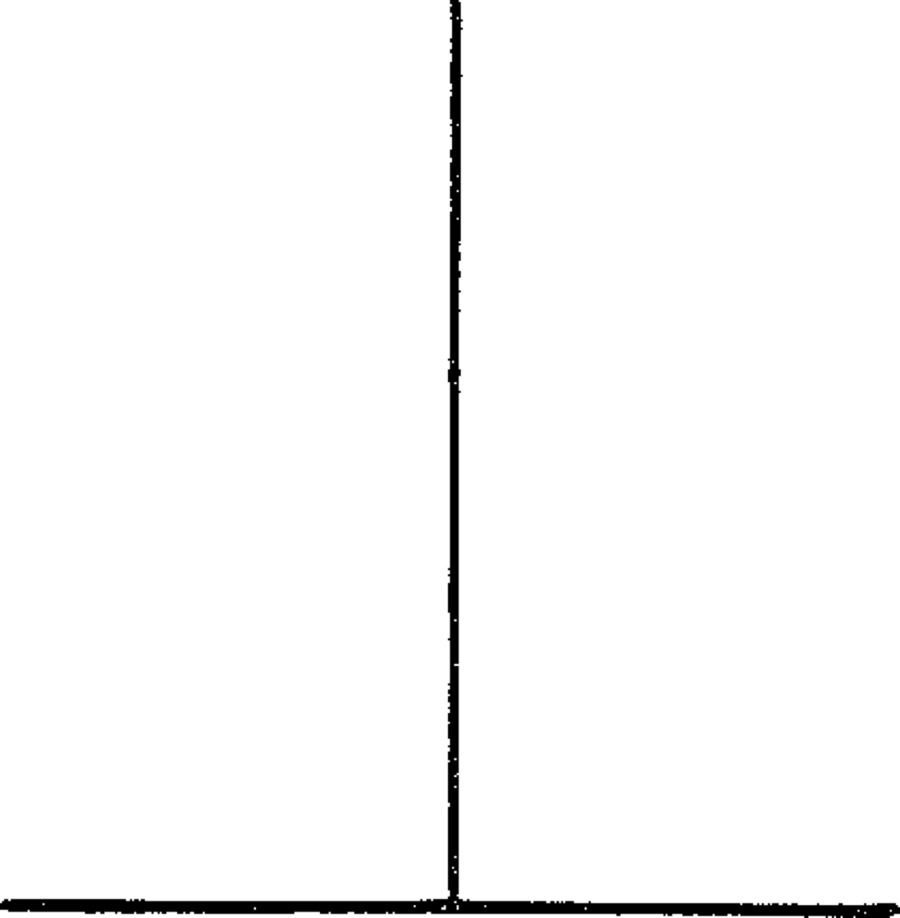
\includegraphics[width=4in]{img/illusions} \par}
	\caption{The sentence for \sysname{Illusions}.}
	\label{illusions}
\end{figure}

\sysname{IIlusions} has Properties 1, 3--5, and 7--8. Purely to clarify this fact, the 
following sequence of integers is presented as a model of the order in which 
associated ratios might appear in reality. (The sequence is otherwise totally 
inadequate as a model of \sysname{Illusions.}) $4 2 1$; $4 2$; $5 4 2 1$; $4 3 1$. The 
implication structure would then be as shown in figure \ref{illusionstructure}.

\begin{figure}
	{\centering 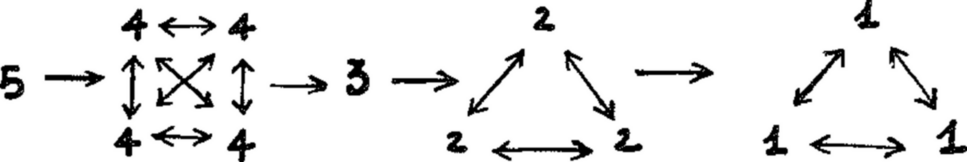
\includegraphics[width=4.5in]{img/illusionstructure} \par}
	\caption{Example implication structure for \sysname{Illusions}.}
	\label{illusionstructure}
\end{figure}

The axiom would be 4, and 5 could not appear in a proof. \sysname{IIlusions} has 
Property 1 on the basis that one can control the associated ratio. Turning to 
Property 4, it is normally the case that when an implication is repeated, a 
given occurrence of one of the sentences involved is unique to a specific 
occurrence of the implication. In \sysname{Illusions,} however, if two equal 
sentences are next smaller than X, the occurrence of X does not uniquely 
belong to either of the two occurrences of the implication. Compare figure \ref{thestructure},
where the occurrence of `$t$' is not unique to either occurrence of `$the$'. 
Subject to this explanation, \sysname{Illusions} has Property 4. \sysname{Illusions} has 
Property 8, but it goes without saying that the type of implication is not 
modus ponens. Properties 3, 5, and 7 need no comment. As for Property 2, 
the rule of implication refers to a property of sentences, rather than to 
elements of sentences. The interesting feature of \sysname{Illusions} is that it 
reverses the situation defined by Properties 6 and 9. Compound indirect 
implication is about the same as simple implication. The only difference is 
the difference between being smaller and being next smaller. And there is 
only one axiom (per person). 

\begin{figure}
	{\centering \begin{tabular}{c c c} t & h & e \\ h &   &   \\ e &   & \end{tabular} \par}
	\caption{Structure with shared node.}
	\label{thestructure}
\end{figure}


Simple direct implication, however, is subjective and illusive. It 
essentially involves changing one's perceptions of an illusion. The change of 
associated ratios is subjective, elusive, and certainly not numerically 
measurable. Then, the order in which one sees sentences won't always be 
their order in the implications and proofs. And even though one is exposed 
to all the sentences, one may have difficulty distinguishing and remembering 
them in consciousness. If I see the normal illusion, then manage to get 
myself to see the lines as being of equal length, I know I have seen a 
theorem. What is difficult is grasping the steps in between, the simple direct 
implications. If the brain contains a permanent impression of every sensation 
it has received, then the implications objectively exist; but they may not be 
thinkable without neurological techniques for getting at the impressions. In 
any case, \enquote{proof} is well-defined in some sense---but proofs may not be 
thinkable. \sysname{Illusions} is, after all, not so much shakier in this respect than 
even simple arithmetic, which contains undecidable sentences and 
indefinable terms. 

In \booktitle{The Logical Syntax of Language}, Carnap distinguishes pure syntax 
and descriptive syntax; and says that pure syntax should be independent of 
notation, and that every system should be isomorphic to some ink-on-paper 
system. In so doing, Carnap violates his own \uline{Principle of Tolerance}. Consider 
the following trivial formalist system. 

\midheading{\enquote{Order}}

\begin{sysrules}
A \enquote{sentence} is a member of a finite set of integers. 

Sentence Y is \enquote{implied by} sentence X if and only if Y=X, or else of all the 
sentences, Y is the one next smaller than X. 

Take as the axiom the largest sentence. 
\end{sysrules}

Is the pure syntax of \sysname{Illusions} isomorphic to \sysname{Order}? The preceding 
paragraph proved that it is not. The implication structure of \sysname{Order} is 
mechanical to the point of idiocy, while the implication structure of 
\sysname{Illusions} is, as I pointed out, elusive. Figure \ref{orderstruc}
where loops indicate multiple occurances of the same sentence, could 
adequately represent a proof in \enquote{Order,} but could not remotely represent 
one in \sysname{Illusions.} The essence of \sysname{Illusions} is that it is coupled to the 
reader's subjectivity. For an ink-on-paper system even to be comparable to 
\sysname{IIlusions,} the subjectivity would have to be moved out of the reader and 
onto the paper. This is utterly impossible. 

\begin{figure}
	{\centering 
\includegraphics[width=4.5in]{img/orderstructure} \par}
	\caption{Implication structure of \sysname{Order}.}
	\label{orderstruc}
\end{figure}

Here is the next system. 

\midheading{\sysname{Innperseqs}}

\begin{sysrules}
Explanation: Consider the rainbow halo which appears to surround a small 
bright light when one looks at it through fogged glass (such as 
eyeglasses which have been breathed on). The halo consists of 
concentric circular bands of color. As the fog evaporates, the halo 
uniformly contracts toward the light. The halo has a vague outer 
ring, which contracts as the halo does. Of concern here is what 
happens on one contracting radius of the halo, and specifically 
what happens on the segment of that radius lying in the vague 
outer ring: the outer segment. 

A \enquote{sentence} (or halopoint) is the changing halo color at a fixed point, in 
space, in the halo; until the halo contracts past the point. 

Several sentences \enquote{imply} another sentence if and only if, at some instant, 
the several sentences are on an outer segment, and the other 
sentence is the inner endpoint of that outer segment. 

An \enquote{axiom} is a sentence which is in the initial vague outer ring (before it 
contracts), and which is not an inner endpoint. 

An \enquote{innperseq} is a sequence of sequences of sentences on one radius 
satisfying the following conditions. 1. The members of the first 
sequence are axioms, 2. For each of the other sequences, the first 
member is implied by the non-first members of the preceding 
sequence; and the remaining inembers (if any) are axioms or first 
members of preceding sequences. 3. All first members, of 
sequences other than the last two, appear as non-first members. 4. 
No sentence appears as a non-first member more than once. 5. The 
last sequence has one member. 
\end{sysrules}


{\centering
\begin{minipage}{1.6in}\imgw{1.3in}{img/innperseqs}\end{minipage}
	\begin{minipage}{2.25in}
\enquote{Sentences} at 

	\begin{tabular}{ c r l }
		\bimg{time1} & $time_1$: & $a_1 a_2 a_3 a_4 a_5 a_6 a_7 b$ \\
		& & $a_1,a_2 \rightarrow\ b$ \\
	\end{tabular}

	\begin{tabular}{c r l}
		\bimg{time2} & $time_2$: & $a_2 a_3 a_4 a_5 a_6 a_7 b c$ \\
		& & $a_3 \rightarrow\ c$ \\
	\end{tabular}

	\begin{tabular}{c r l}
		\bimg{time3} & $time_3$: & $a_4 a_5 a_6 a_7 b c d$ \\
		& & $a_4,a_5 \rightarrow\ d$ \\
	\end{tabular}

	\begin{tabular}{c r l}
		\bimg{time4} & $time_4$: & $a_6 a_7 b c d e$ \\
		& & $a_6,b \rightarrow\ e$ \\
	\end{tabular}

	\begin{tabular}{c r l}
		\bimg{time5} & $time_5$: & $a_7 b c d e f$ \\
		& & $a_7,c \rightarrow\ f$ \\
	\end{tabular}

	\begin{tabular}{c r l}
		\bimg{time6} & $time_6$: & $c d e f g$ \\
		& & $d,e \rightarrow\ g$ \\
	\end{tabular}

\enquote{Axioms} $a_1 a_2 a_3 a_4 a_5 a_6 a_7$


Innperseq \\
$(a_3,a_2,a_1)$
$(b,a_3)$
$(c,a_5,a_4)$
$(d,b,a_6)$
$(e,c,a_7)$
$(f,e,d)$
$(g)$
	\end{minipage}\par}

In the diagram, different positions of the vague outer 
ring at different times are suggested by different shadings. The 
outer segment moves \enquote{down the page.} The figure is by no means 
an innperseq, but is supposed to help explain the definition. 
In \sysname{Innperseqs,} a conventional proof would be redundant unless all 
the statements were on the same radius. And even if the weakest axiom were 
chosen (the initial outer endpoint), this axiom would imply the initial inner 
endpoint, and from there the theorem could be reached immediately. In 
other words, to use the standard definition of \enquote{proof} in \sysname{Innperseqs} 
would result in an uninteresting derivation structure. Thus, a more 
interesting derivation structure is defined, the \enquote{\term{innperseq.}} The interest of 
an \enquote{\term{innperseq}} is to be as elaborate as the many restrictions in its definition 
will allow. Proofs are either disregarded in \sysname{Innperseqs}; or else they are 
identified with innperseqs, and lack Property 8. \sysname{Innperseqs} makes the 
break with the proof-theorem structure of formalist mathematics. 

Turning to simple implication, an implicand can have many impliors; 
and there is an infinity of axioms, specified by a general condition. The 
system has Property 1 in the sense that a sentence can exist at different 
times and be a member of different implications. It has Property 4 in the 
sense that the sentences in a specific implication can exist at different times, 
and the implication holds as long as the sentences exist. It has Property 3 in 
that an inner endpoint implies itself. The system also has Properties 5 and 7; 
and lacks Property 2. But, as before, Properties 6 and 9 are another matter. 
Given several sentences, it is certainly possible to tell mechanically whether 
one is implied by the others. But when are you given sentences? If one can 
think the sentences, then relating them is easy---but it is difficult to think the 
sentences in the first place, even though they objectively exist. The diagram 
suggests what to look for, but the actual thinking, the actual sentences are 
another matter. As for Property 9, when \enquote{theorems} are identified with last 
members of innperseqs, I hesitate to say whether a derivation of a given 
sentence can be constructed mechanically. If a sentence is nearer the center 
than the axioms are, an innperseq can be constructed for it. Or can it? The 
answer is contingent. \enquote{Innperseqs} is indeterminate because of the difficulty 
of thinking the sentences, a difficulty which is defined into the system. It is 
the mathematician's capabilities at a particular instant which delimit the 
indeterminacies. Precisely because of the difficulty of thinking sentences, I 
will give several subvariants of the system. 

\midheading{Indeterminacy}

\begin{sysrules}
A \enquote{totally determinate innperseq} is an innperseq in which one thinks all the 
sentences. 

An \enquote{implior-indeterminate innperseq} is an innperseq in which one thinks 
only each implicand and the outer segment it terminates. 

A \enquote{sententially indeterminate innperseq} is an innperseq in which one thinks 
only the outer segment, and its inner endpoint, as it progresses 
inward. 
\end{sysrules}


Let us return to the matter of pure and descriptive syntax. The interest 
of \enquote{Illusions} and \enquote{Innperseqs} is precisely that their abstract structure 
cannot be separated from their physical and psychological character, and 
thus that they are not isomorphic to any conventional ink-on-paper system. I 
am trying to break through to unheard of, and hopefully significant, modes 
of implication; to define implication structures (and derivation structures) 
beyond the reach of past mathematics. 

\subsection{Constructed Memory Systems}

In order to understand this section, it is necessary to be thoroughly 
familiar with \essaytitle{Studies in Constructed Memories,} the essay following this 
one. (I have not combined the two essays because their approaches are too 
different.) I will define post-formalist systems in constructed memories, 
beginning with a system in an M*-Memory. 

\midheading{\enquote{Dream Amalgams}}

\begin{sysrules}
A \enquote{sentence} is a possible method, an $A_{a_i}$. with respect to an M*-Memory. 
The sentence $A_{a_p}$ \enquote{implies} the sentence $A_{a_q}$ if and only if the $a_q$th 
M*-assertion is actually thought; and either $A_{a_q} = A_{a_p}$, or else there is 
cross-method contact of a mental state in $A_{a_q}$ with a state in $A_{q_p}$\footnote{sic?}

The axioms must be chosen from sentences which satisfy two conditions. 
The mental states in the sentences must have cross-method contact 
with mental states in other sentences. And the M*-assertions 
corresponding to the sentences must not be thought. 

Explanation: As \essaytitle{Studies in Constructed Memories} says, there can be 
cross-method contact of states, because a normal dream can 
combine totally different episodes in the dreamer's life into an 
amalgam. 
\end{sysrules}

\enquote{\textsc{Dream Amalgams}} has Properties 1--5. For the first time, sentences are 
structurally composite, with mental states being the relevant sentential 
elements. Implication has an unusual character. The traditional type of 
implication, modus ponens, is \enquote{directed,} because the conditional is 
directed. Even if $\ulcorner\varphi\supset\phi\urcorner$ is true 
$\ulcorner\varphi\supset\phi\urcorner$ may not be. Now implication is also 
directed in \enquote{\textsc{Dream Amalgams,}} but for a very different reason. 
Cross-method contact, unlike the conditional, has a symmetric character. 
What prevents implication from being necessarily symmetrical is that the 
implicand's M*-assertion actually has to be thought, while the implior's 
M*-assertion does not. Thus, implication is both subjective and mechanical, 
it is subjective, in that it is a matter of volition which method is remembered 
to have actually: been used. It is mechanical, in that when one is 
remembering, one is automatically aware of the cross-method contacts of 
states in $A_{a_q}$. The conditions on the axioms ensure that they will have 
implications without losing Property 7. 

As for compound implication in \enquote{\textsc{Dream Amalgams,}} the organism 
with the M*-Memory can't be aware of it at all; because it can't be aware 
that at different times it remembered different methods to be the one 
actually used. (In fact, the organism cannot be aware that the system has 
Property 5, for the same reason.) On the other hand, to an outside observer 
of the M*-Memory, indirect implication is not only thinkable but 
mechanical. It is not superfluous because cross-method contact of mental 
states is not necessarily transitive. The outside observer can decide whether a 
sentence is a theorem by the following mechanical procedure. Check 
whether the sentence's M*-assertion has acually been thought; if so, check all 
sentences which imply it to see if any are axioms; if not, check all the 
sentences which imply the sentences which imply it to see if any are axioms; 
etc. The number of possible methods is given as finite, so the procedure is 
certain to terminate. Again, an unprecedented mode of implication has been 
defined. 

When a post-formalist system is defined in a constructed memory, the 
discussion and analysis of the system become a consequence of constructed 
memory theory and an extension of it. Constructed memory theory, which 
is quite unusual but still more or less employs deductive inference, is used to 
study post-formalist modes of inference which are anything but deductive. 

To aid in understanding the next system, which involves infalls in a 
D-Memory, here is an 

{ \vskip 1.5em \centering \large \framebox[1.1\width]{\enquote{Exercise to be Read Aloud}} \par\vskip 1.5em}

(Read according to a timer, reading the first word at O' O", and prolonging 
and spacing words so that each sentence ends at the time in parentheses after 
it. Do not pause netween sentences.) 

\begin{tabular}{ r p{2.5in} }
	($event_1$) &  All men are mortal. (17") \\

	($Sentence_1=event_2s$) &  The first utterance lasted 17" and ended at 17"; and lasted 15" and ended 1" ago. (59") \\

	($S_2=event_3$) & The second utterance lasted 42" and ended at 59": and lasted 50" and ended 2" ago. (1' 31") \\

	($S_3=event_4$) & The third utterance lasted 32" and ended at 1' 31"; and lasted 40" and ended 1" ago. (2' 16") \\
\end{tabular}

Since '32' in $S_3$ is greater than '2' in $S_2$, $S_2$ must say that $S_1$ ($=event_2$)
ended 30" after $S_2$ began, or something equally unclear. The duration of $S_2$
is greater than the distance into the past to which it refers. This situation is 
not a real infall, but it should give the reader some intuitive notion of an 
infall. 

\midheading{"Infalls"}

\begin{sysrules}
	A "sentence" is a D-sentence, in a D-Memory such that $event_{j+1}$ is the first 
thinking of the jth D-sentence, for all j. 

Two sentences "imply" another if and only if all three are the same; or else 
the three are adjacent (and can be written $S_{j+1},S_j,S_{j-1}$), and are such 
that $\delta_j=x_{j+1}-x_j> z_j,$ $S^D_{j-1}$ is the implicand. (The function of $S_{j+1}$ is to 
give the duration $\delta_j=x_{j+1}-x_j$ of $S_j$. $S_j$ states that $event_j$, the first 
thinking of $S^{D}_{j-1}$, ended at a distance $z_j$ into the past, where $z_j$ is smaller 
than $S^D_j$'s own duration. The diagram indicates the relations.) 
\end{sysrules}

\imgw{4in}{img/infallsdiag}

In this variety of D-Memory, the organism continuously thinks successive 
D-sentences, which are all different, just as the reader of the above exercise 
continuously reads successive and different sentences. Thus, the possibility 
of repeating a sentence depends on the possibility of thinking it while one is 
thinking another sentence---a possibility which may be far-fetched, but which 
is not explicitly excluded by the definition of a "D-Memory." If the 
possibility is granted, then "\textsc{Infalls}" has Properties 1--5. Direct implication is 
completely mechanical; it is subjective only in that the involuntary 
determination of the $z_j$ and other aspects of the memory is a 'subjective' 
process of the organism. Compound implication is also mechanical to an 
outside observer of the memory, but if the organism itself is to be aware of 
it, it has to perform fantastic feats of multiple thinking. 

"\textsc{Dream Amalgams}" and "\textsc{Infalls}" are systems constructed with 
imaginary elements, systems whose "notation" is drawn from an imaginary 
object or system. Such systems have no descriptive syntax. Imaginary objects 
were introduced into mathematics, or at least into geometry, by Nicholas 
Lobachevski, and now I am using them as a notation. For these systems to 
be nonisomorphic to any ink-on-paper systems, the mathematician must be 
the organism with the M*-Memory or the D*-Memory. But this means that 
in this case, the mathematics which is nonisomorphic to any ink-on-paper 
system can be performed only in an imaginary mind. 

Now for a different approach. Carnap said that we are free to choose 
the rules of a system arbitrarily. Let us take Carnap literally. I want to 
construct more systems in constructed memories---so why not construct the 
system by a procedure which ensures that constructed memories are 
involved, but which is otherwise arbitrary? Why not suspend the striving 
after "interesting" systems, that last vestige of the striving after 
"correctness," and see what happens? Why not construct the rules of a 
system by a chance procedure? 

To construct a system, we have to fill in the blanks in the following rule 
schema in such a way that grammatically correct sentences result. 

\newcommand{\blankspace}{\_\_\_\_\_\_\_\_\_\_}

\midheading{Rule Schema}

\begin{sysrules}
A "sentence" is a(n) \blankspace.

Two sentences "imply" a third if and only if the two sentences \blankspace\ the third. 

An "axiom" is a sentence that \blankspace.
\end{sysrules}


I now spread the pages of \essaytitle{Studies in Constructed Memories} on the floor. 
With eyes closed, I hold a penny over them and drop it. I open my eyes and 
copy down the expressions the penny covers. By repeating this routine, I 
obtain a haphazard series of expressions concerning constructed memories. It 
is with this series that I will fill in the blanks in the rule schema. In the next 
stage, I fill the first (second, third) blank with the ceries of expressions 
preceding the-first (second, third) period in the entire series. 

\midheading{"Haphazard System"}

\begin{sysrules}
A "sentence" is a the duration D-sentences $\triangle\ (\mathparagraph^m)$ conclude these 
"$\Phi^*$-Reflec\-tion," or the future Assumption voluntarily force of 
conviction for conclusion the Situation or by ongoing that this 
system? be given telling between the Situation 1. 

Two sentences "imply" a third if and only if the two sentences is\slash was 
contained not have to the acceptance that a certain and malleable 
study what an event involves material specifically mathematics: 
construct accompanies the rest, extra-linguistically image organism 
can fantasy not remembering $\Phi^*$-Memory, the future interval defined 
in dream the third. 

An "axiom" is a sentence that internally D-sentences, just as the 
"$\Phi^*$-Memory" sentences $A_{a_1}$ is $A_{a_2}$. 

In the final stage, I cancel the smallest number of words I have to in 
order to make the rules grammatical. 
\end{sysrules}

\midheading{"Fantasied Amnesia"}

\begin{sysrules}
A "sentence" is a duration or the future force of conviction for the Situation 
or this system given Situation 1. 

Two sentences "imply" a third if and only if the two sentences have the 
acceptance that a certain and malleable study extra-linguistically can 
fantasy not remembering the future interval defined in the third. 

An "axiom" is a sentence that internally just sentences $A_{a_2}$.
\end{sysrules}

It becomes clear in thinking about "Fantasied Amnesia" that its 
metametamathematics is dual. Describing the construction of the rules, the 
metamathematics, by a systematic performance, is one thing. Taking the 
finished metamathematics at face value, independently of its origin, and 
studying it in the usual manner, is another. Let us take "Fantasied Amnesia" 
at face value. As one becomes used to its rules, they become somewhat more 
meaningful. I will say that an "interpretation" of a haphazard system is an 
explanation of its rules that makes some sense out of what may seem 
senseless. "Interpreting" is somewhat like finding the conditions for the 
existence of a constructed memory which seemingly cannot exist. The first 
rule of "Fantasied Amnesia" is a disjunction of three substantives. The 
"Situation" referred to in the second substantive expression is either 
Situation 1 or else an unspecified situation. The third substantive expression 
apparently means "this system, assuming Situation 1," and refers to 
"Fantasied Amnesia" itself. The definition of "sentence" is thus meaningful, 
but very bizarre. The second rule speaks of "the acceptance" as if it were a 
written assent. The rule then speaks of a "malleable study" as "fantasying" 
something. This construction is quite weird, but let us try to accept it. The 
third rule speaks of a sentence that "sentences" (in the legal sense) a possible 
method. So much for the meaning of the rules. 

Turning to the nine properties of formalist systems, the reference to 
"the future interval" in the implication rule of "Fantasied Amnesia" 
indicates that the system has Property 2; and the system can perfectly well 
have Property 8. It does not have Property 6 in any known sense. Certainly 
it does have Property 9. it just might have Property. 1. But as for the other 
four properties, it seems out of the question to decide whether "Fantasied 
Amnesia" has them. For whatever it is worth, "Fantasied Amnesia" is on 
balance incomparable to formalist systems. 

My transformation rule schema has the form of a biconditional, in 
which the right clause is the operative one. If a transformation rule were to 
vary, in such a way that it could be replaced by a constant rule whose right 
clause was the disjunction of the various right clauses for the variable rule, 
then the latter would vary "trivially." 1 will say that a system whose 
transformation rule can vary non-trivially is a "heterodeterminate" system. 
Since 1 have constructed a haphazard metamathematics, why not a 
heterodeterminate metamathematics? Consider a mathematician with an 
M-Memory, such that each $A_{a_i}$. is the consistent use of a different 
transformation rule, a different definition of "imply," for the mathematics 
in which the mathematician is discovering theorems. The consistent use of a 
transformation rule is after all a method---a method for finding the 
commitments premisses make, and for basing conclusions in premisses. When 
the mathematician goes to remember which rule of inference he has actually 
been using, he "chooses" which of the possible methods is remembered to 
have actually been used. This situation amounts to a heterodeterminate 
system. tn fact, the metamathematics cannot even be written out this time; I 
can only describe it metametamathematically in terms of an imaginary 
memory. 

We are now in the realm of mathematical systems which cannot be 
written out, but can only be described metametamathematically. I will 
present a final system of this sort. It is entitled \textsc{"System Such That No One 
Knows What's Going On."} One just has to guess whether this system exists, 
and if it does what it is like. The preceding remark is the 
metametamathematical description, or definition, of the system. 

\subsection{Epilogue}

Ever since Carnap's Principle of Tolerance opened the floodgates to 
arbitrariness in mathematics, we have been faced with the prospect of a 
mathematics which is  indistinguishable from  art-for-art's-sake, or 
amusement-for-amusement's-sake. But there is one characteristic which saves 
mathematics from this fate. Mathematics originated by abstraction from 
primitive technology, and is indispensable to science and technology---in 
short, mathematics has scientific applications. The experience of group 
theory has proved, I hope once and for all, the bankruptcy of that narrow 
practicality which would limit mathematics to what can currently be applied 
in science. But now that mathematics is wide open, and anything goes, we 
should be aware more than ever that scientific applicability is the only 
objective value that mathematics has. I would not have set down constructed 
memory theory and the post-formalist systems if I did not believe that they 
could be applied. When and how they will be is another matter. 

And what about the "validity" of formalism? The rise of the formalist 
position is certainly understandable. The formalists had a commendable, 
rationalistic desire to eliminate the metaphysical problems associated with 
mathematics. Moreover, formalism helped stimulate the development of the 
logic needed in computer technology (and also to stimulate this paper). In 
spite of the productiveness of the formalist position, however, it now seems 
beyond dispute that formalism has failed to achieve its original goals. (My 
pure philosophical writings are the last word on this issue.) Perhaps the main 
lesson to be learned from the history of formalism is that an idea does not 
have to be "true" to be productive. 


\section*{Note}
Early versions of \textsc{"Illusions"} and \textsc{"Innperseqs"} appeared in my essay 
"Concept Art," published in An Anthology, ed. La Monte Young, New 
York, 1963. An early, July 1961 version of \textsc{"System Such That No One 
Knows What's Going On"} appeared in dimension 14, Ann Arbor, 1963, 
published by the University of Michigan College of Architecture and Design. 

